\documentclass[11pt]{article}
\usepackage[utf8]{inputenc}
\usepackage[french]{babel}
\usepackage[T1]{fontenc}
\usepackage{verbatim}
\usepackage{graphicx}
\usepackage{amsmath}
\usepackage{eurosym}
\usepackage{textcomp}
\usepackage{graphicx}
\author{Contzen Laurent, Corvalan Gabriel}
\title{NaluRSS}
\date{14 Décembre 2009}

\begin{document}

\begin{titlepage}
\begin{flushleft}
Contzen Laurent \\
Corvalan Gabriel \\
\end{flushleft}
\begin{center}
\vspace{65mm}\LARGE{\textbf{INFO-H-303 - Bases de données} :\\
NaluRSS}
\end{center}
\begin{flushright}
\vspace{70mm}
Année Académique 2009-2010.
\end{flushright}
\end{titlepage}
\tableofcontents
\newpage

\section{Introduction}
Dans le cadre de ce projet du cours de bases de données nous avons du développer un agrégateur de flux rss. Un flux rss est un fichier xml\footnote{eXtensible Markup Language} contenant des informations sur les dernières mises à jour d'un site internet. Une fois ce flux intégré dans un agrégateur l'utilisateur est automatiquement tenu au courant de ces mises à jour. Le grand intérêt de ceci est de pouvoir avoir les nouvelles ionformations de tous nos sites préférés en une fois dans une seule même interface plutot que de devoir aller sur chaque site un à un.
\section{Présentation de NaluRSS}
NaluRSS est entièrement écrit en xhtml\footnote{eXtensible HyperText Markup Language}/css\footnote{Cascading Style Sheet} et php\footnote{PHP: HyperText Preprocessor} et enregistre les informations dans une base de données MySQL. Il a été pensé pour être le plus simple d'utilisation possible pour l'utilisateur. Ses principales fonctionnalités sont :
\begin{itemize}
\item{Un système multi-utilisateurs}
\item{La possibilité d'être \og ami \fg avec un autre utilisateur}
\item{La possibilité de partager une nouvelle d'un flux avec ses \og amis \fg, et ce avec un commentaire}
\item{La possibilité d'ajouter ou supprimer des \og amis \fg}
\item{L'ajout et la suppression de feeds}
\item{L'affichage des flux en version condensée (juste les titres des articles) ou en version complète (les titres et descriptions des articles)}
\item{L'affichage des flux des \og amis \fg (chaque élément partagé par une personne fait partie de son flux personnel)}*
\item{L'affichage d'un unique article avec sa description}
\item{La possibilité de s'inscrire sur le site}
\item{Et bien d'autres}
\end{itemize}
Voici une capture d'écran de la page d'accueil :
\begin{figure}[!ht]
\begin{center}
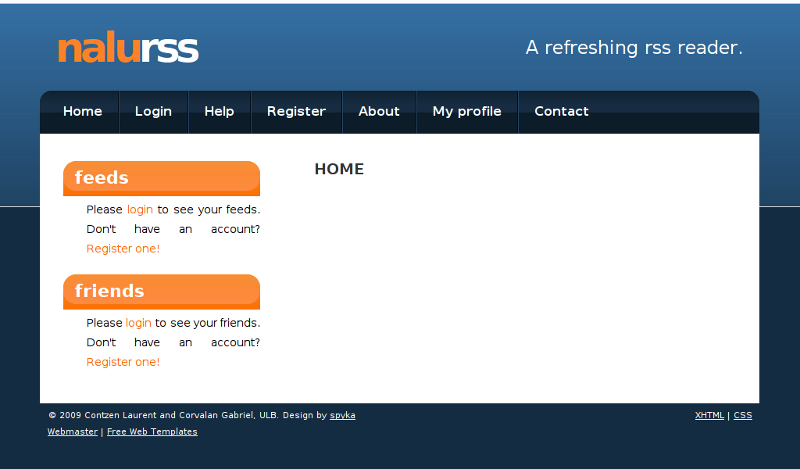
\includegraphics[width=14cm]{home.png}
\end{center}
\caption{Page d'accueil de NaluRSS pour un utilisateur non enregistré}
\label{home}
\end{figure}
\newline

\section{Script SQL DDL de création de la base de données}

\section{Requêtes demandés en algèbre relationnel}
\subsection{R1}
\noindent $AcceptedFriends \longleftarrow \pi_{EmailA, EmailB}(\sigma_{Accepted = 1}(Friends))$ \\
$UsersMails \longleftarrow \pi_{Email}(Users)$ \\
$temp \longleftarrow AcceptedFriends \ast \alpha_{EmailB : EmailC}(AcceptedFriends) \ast \alpha_{EmailB : EmailD}(AcceptedFriends) $ \\
$temp2 \longleftarrow \alpha_{EmailA : Email}(\pi_{EmailA}(\sigma_{EmailB \neq EmailC \wedge EmailB \neq EmailD \wedge EmailC \neq EmailD}(temp))) $ \\
$Result \longleftarrow UsersMails - temp2 $
\subsection{R2}
\noindent $FeedsX \longleftarrow \pi_{Email = X}(Subscriptions) $ \\

\subsection{R3}
\noindent $FeedsX \longleftarrow \pi_{Email = X}(Subscriptions) $ \\
$SharesX \longleftarrow \pi_{Email}(\sigma_{Email = X}(Shares))$ \\
$FriendsX \longleftarrow \alpha_{EmailA : Email}(\pi_{EmailA}(\sigma_{EmailA = X \wedge Accepted = 1}(Friends))) \cup \alpha_{EmailB : Email} (\pi_{EmailB}(\sigma_{EmailB = X \wedge Accepted = 1}(Friends)))$ \\
$Result \longleftarrow FeedsX - FriendsX - SharesX$
\subsection{R4}


\section{Requêtes demandés en calcul relationnel tuple}
\subsection{R1}

\subsection{R2}

\subsection{R3}

\subsection{R4}

\section{Requêtes demandés en SQL}
\subsection{R1}

\subsection{R2}

\subsection{R3}

\subsection{R4}

\subsection{R5}

\subsection{R6}



\section{Instructions d'installation}
\subsection{Pré-requis}
Afin d'installer NaluRSS il faut disposer d'un serveur sur lequel tournent un serveur web\footnote{Apache par exemple}, une base de données MySQL et un interpréteur PHP. Tout ceci se trouve facilement sur la plupart des hébergeurs ou s'installe très facilement en tant que serveur LAMP\footnote{Linux Apache Mysql Php}, WAMP\footnote{Windows Apache Mysql Php} ou encore MAMP\footnote{Mac Apache Mysql Php}. Le programme phpMyAdmin peut aussi être installé pour faciliter les interactions manuelles avec la base de données.
\subsection{Installation}
Une fois que nous avons un serveur *AMP fonctionnel en marche l'installation est extrèmement simple : il suffit de 
\begin{itemize}
\item{Décompresser l'archive dans le répertoire fixé par la configuration du serveur Apache}
\item{Importer la structure de données}
\end{itemize}

\section{Scénario de démonstration}

\section{Explications diverses}

\section{Conclusion}
Nous avons donc ici un agrégateur de flux rss parfaitement utilisable en production si les fonctionnalités présentes suffisent, et facilement extensible à souhait sinon.
\end{document}
